\documentclass{IEEEtran4PSCC}

\ifCLASSINFOpdf
  \usepackage[pdftex]{graphicx}
  % declare the path(s) where your graphic files are
  % \graphicspath{{../pdf/}{../jpeg/}}
  % and their extensions so you won't have to specify these with
  % every instance of \includegraphics
  % \DeclareGraphicsExtensions{.pdf,.jpeg,.png}
\else
  % or other class option (dvipsone, dvipdf, if not using dvips). graphicx
  % will default to the driver specified in the system graphics.cfg if no
  % driver is specified.
  \usepackage[dvips]{graphicx}
  % declare the path(s) where your graphic files are
  % \graphicspath{{../eps/}}
  % and their extensions so you won't have to specify these with
  % every instance of \includegraphics
  % \DeclareGraphicsExtensions{.eps}
\fi
% graphicx was written by David Carlisle and Sebastian Rahtz. It is
% required if you want graphics, photos, etc. graphicx.sty is already
% installed on most LaTeX systems. The latest version and documentation
% can be obtained at: 
% http://www.ctan.org/tex-archive/macros/Latex/required/graphics/
% Another good source of documentation is 'Using Imported Graphics in
% LaTeX2e' by Keith Reckdahl which can be found at:
% http://www.ctan.org/tex-archive/info/epsLatex/
%
% Latex, and pdfLatex in dvi mode, support graphics in encapsulated
% postscript (.eps) format. pdfLatex in pdf mode supports graphics
% in .pdf, .jpeg, .png and .mps (metapost) formats. Users should ensure
% that all non-photo figures use a vector format (.eps, .pdf, .mps) and
% not a bitmapped formats (.jpeg, .png). IEEE frowns on bitmapped formats
% which can result in 'jaggedy'/blurry rendering of lines and letters as
% well as large increases in file sizes.
%
% You can find documentation about the pdfTeX application at:
% http://www.tug.org/applications/pdftex


\usepackage[cmex10]{amsmath}





% *** SPECIALIZED LIST PACKAGES ***
%
% \usepackage{algorithmic}
% algorithmic.sty was written by Peter Williams and Rogerio Brito.
% This package provides an algorithmic environment fo describing algorithms.
% You can use the algorithmic environment in-text or within a figure
% environment to provide for a floating algorithm. Do NOT use the algorithm
% floating environment provided by algorithm.sty (by the same authors) or
% algorithm2e.sty (by Christophe Fiorio) as IEEE does not use dedicated
% algorithm float types and packages that provide these will not provide
% correct IEEE style captions. The latest version and documentation of
% algorithmic.sty can be obtained at:
% http://www.ctan.org/tex-archive/macros/Latex/contrib/algorithms/
% There is also a support site at:
% http://algorithms.berlios.de/index.html
% Also of interest may be the (relatively newer and more customizable)
% algorithmicx.sty package by Szasz Janos:
% http://www.ctan.org/tex-archive/macros/Latex/contrib/algorithmicx/




% *** ALIGNMENT PACKAGES ***
%
%\usepackage{array}
% Frank Mittelbach's and David Carlisle's array.sty patches and improves
% the standard LaTeX2e array and tabular environments to provide better
% appearance and additional user controls. As the default LaTeX2e table
% generation code is lacking to the point of almost being broken with
% respect to the quality of the end results, all users are strongly
% advised to use an enhanced (at the very least that provided by array.sty)
% set of table tools. array.sty is already installed on most systems. The
% latest version and documentation can be obtained at:
% http://www.ctan.org/tex-archive/macros/Latex/required/tools/


% IEEEtran contains the IEEEeqnarray family of commands that can be used to
% generate multiline equations as well as matrices, tables, etc., of high
% quality.




% *** SUBFIGURE PACKAGES ***
%\ifCLASSOPTIONcompsoc
%  \usepackage[caption=false,font=normalsize,labelfont=sf,textfont=sf]{subfig}
%\else
%  \usepackage[caption=false,font=footnotesize]{subfig}
%\fi
% subfig.sty, written by Steven Douglas Cochran, is the modern replacement
% for subfigure.sty, the latter of which is no longer maintained and is
% incompatible with some LaTeX packages including fixltx2e. However,
% subfig.sty requires and automatically loads Axel Sommerfeldt's caption.sty
% which will override IEEEtran.cls' handling of captions and this will result
% in non-IEEE style figure/table captions. To prevent this problem, be sure
% and invoke subfig.sty's 'caption=false' package option (available since
% subfig.sty version 1.3, 2005/06/28) as this is will preserve IEEEtran.cls
% handling of captions.
% Note that the Computer Society format requires a larger sans serif font
% than the serif footnote size font used in traditional IEEE formatting
% and thus the need to invoke different subfig.sty package options depending
% on whether compsoc mode has been enabled.
%
% The latest version and documentation of subfig.sty can be obtained at:
% http://www.ctan.org/tex-archive/macros/Latex/contrib/subfig/




% *** FLOAT PACKAGES ***
%
%\usepackage{fixltx2e}
% fixltx2e, the successor to the earlier fix2col.sty, was written by
% Frank Mittelbach and David Carlisle. This package corrects a few problems
% in the LaTeX2e kernel, the most notable of which is that in current
% LaTeX2e releases, the ordering of single and double column floats is not
% guaranteed to be preserved. Thus, an unpatched LaTeX2e can allow a
% single column figure to be placed prior to an earlier double column
% figure. The latest version and documentation can be found at:
% http://www.ctan.org/tex-archive/macros/Latex/base/


%\usepackage{stfloats}
% stfloats.sty was written by Sigitas Tolusis. This package gives LaTeX2e
% the ability to do double column floats at the bottom of the page as well
% as the top. (e.g., '\begin{figure*}[!b]' is not normally possible in
% LaTeX2e). It also provides a command:
%\fnbelowfloat
% to enable the placement of footnotes below bottom floats (the standard
% LaTeX2e kernel puts them above bottom floats). This is an invasive package
% which rewrites many portions of the LaTeX2e float routines. It may not work
% with other packages that modify the LaTeX2e float routines. The latest
% version and documentation can be obtained at:
% http://www.ctan.org/tex-archive/macros/Latex/contrib/sttools/
% Do not use the stfloats baselinefloat ability as IEEE does not allow
% \baselineskip to stretch. Authors submitting work to the IEEE should note
% that IEEE rarely uses double column equations and that authors should try
% to avoid such use. Do not be tempted to use the cuted.sty or midfloat.sty
% packages (also by Sigitas Tolusis) as IEEE does not format its papers in
% such ways.
% Do not attempt to use stfloats with fixltx2e as they are incompatible.
% Instead, use Morten Hogholm'a dblfloatfix which combines the features
% of both fixltx2e and stfloats:
%
% \usepackage{dblfloatfix}
% The latest version can be found at:
% http://www.ctan.org/tex-archive/macros/Latex/contrib/dblfloatfix/




% *** PDF, URL AND HYPERLINK PACKAGES ***
%
% \usepackage{url}
% url.sty was written by Donald Arseneau. It provides better support for
% handling and breaking URLs. url.sty is already installed on most LaTeX
% systems. The latest version and documentation can be obtained at:
% http://www.ctan.org/tex-archive/macros/Latex/contrib/url/
% Basically, \url{my_url_here}.


% correct bad hyphenation here
\hyphenation{op-tical net-works semi-conduc-tor}



% Set footer
\makeatletter
\let\old@ps@headings\ps@headings
\let\old@ps@IEEEtitlepagestyle\ps@IEEEtitlepagestyle
\def\psccfooter#1{%
    \def\ps@headings{%
        \old@ps@headings%
        \def\@oddfoot{\strut\hfill#1\hfill\strut}%
        \def\@evenfoot{\strut\hfill#1\hfill\strut}%
    }%
    \def\ps@IEEEtitlepagestyle{%
        \old@ps@IEEEtitlepagestyle%
        \def\@oddfoot{\strut\hfill#1\hfill\strut}%
        \def\@evenfoot{\strut\hfill#1\hfill\strut}%
    }%
    \ps@headings%
}
\makeatother

\psccfooter{%
        \parbox{\textwidth}{\hrulefill \\ \small{23rd Power Systems Computation Conference} \hfill \begin{minipage}{0.2\textwidth}\centering \vspace*{4pt} 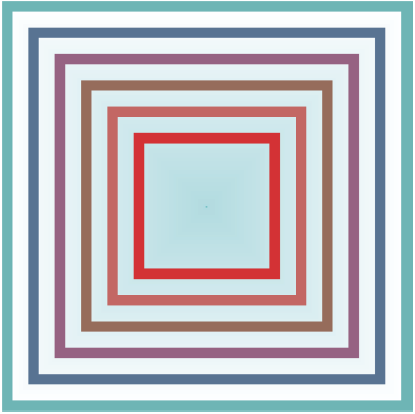
\includegraphics[scale=0.06]{PSCC_logo.png}\\\small{PSCC 2024} \end{minipage} \hfill \small{Paris-Saclay France --- June 04 -- June 07, 2024}}%
}

\usepackage{lipsum}
\usepackage{import}
\usepackage{standalone}
\usepackage{dirtree}

\begin{document}

\newcommand{\imagedir}{../images}
\newcommand{\figdir}{../figures}

\newcommand{\packageName}{PowerEdu.jl}
\providecommand{\packageNameNoJL}[1]{PowerEdu}
\providecommand{\powerflow}[1]{Power Flow}
\providecommand{\sparse}[1]{Sparse Power Flow}
\providecommand{\cpf}[1]{Continuation Power Flow}
\providecommand{\se}[1]{State Estimation}
\providecommand{\opf}[1]{Optimal Power Flow}

\title{\packageName{} - A Julia Package for Teaching Power System Courses}



%% To specify the authors when (number of affiliations <= 2)
\author{
% \IEEEauthorblockN{Ninad Gaikwad, Aryan Jha, Sajjad Uddin Mahmud, Anamika Dubey, Noel Schulz, and Mani Venkatasubramanian}
\IEEEauthorblockN{Ninad Gaikwad, Aryan Jha, Sajjad Uddin Mahmud and Anamika Dubey}
\IEEEauthorblockA{School of Electrical Engineering \& Computer Science, Washington State University, Pullman, WA, USA\\
% \{ninad.gaikwad, aryan.jha, sajjaduddin.mahmud, anamika.dubey, noel.schulz, mani\}@wsu.edu}
\{ninad.gaikwad, aryan.jha, sajjaduddin.mahmud, anamika.dubey\}@wsu.edu}
}

%% To specify the authors when (number of affiliations > 2)
% \author{\IEEEauthorblockN{Author n.1\IEEEauthorrefmark{1},
% Author n.2\IEEEauthorrefmark{2},
% Author n.3\IEEEauthorrefmark{3}, 
% Author n.4\IEEEauthorrefmark{3} and
% Author n.5\IEEEauthorrefmark{4}}
% \IEEEauthorblockA{\IEEEauthorrefmark{1} Department Name of Organization A\\
% Name of the organization A,
% Address A\\ Emails if wanted}
% \IEEEauthorblockA{\IEEEauthorrefmark{2} Department Name of Organization B\\
% Name of the organization B,
% Address B\\ Emails if wanted}
% \IEEEauthorblockA{\IEEEauthorrefmark{3} Department Name of Organization C\\
% Name of the organization C,
% Address C\\ Emails if wanted}
% \IEEEauthorblockA{\IEEEauthorrefmark{4}Department Name of Organization D\\
% Name of the organization D,
% Address D\\ Emails if wanted}
% }


\maketitle

\begin{abstract}
  % \documentclass[class=IEEEtran4PSCC]{standalone}
% \documentclass[article]{standalone}
\documentclass{article}
\ifdefined\packageName
\else
    \newcommand{\packageName}[1]{PowerEdu.jl}
\fi

\begin{document}
    We introduce PowerEdu.jl, an open-source, beginner-friendly package in the Julia
    programming language designed for budding power system engineers. This package 
    addresses the current gap in accessible and comprehensive tools for transmission network
    computations. PowerEdu.jl covers Power Flow using innovative dense 
    and sparse data structures, Continuation Power Flow, State Estimation, Optimal 
    Power Flow, Small-Signal Stability, and Transient Stability Analysis. Notably, 
    the package is scalable, allowing for analysis of systems of varying 
    sizes. User interaction with component modules is highly customizable; for example, 
    users can opt to print detailed intermediary steps, such as Jacobians and mismatches, 
    in Power Flow calculations. We use DataFrames for intuitive and visually 
    appealing data representation. In this paper, we detail the key modules of 
    PowerEdu.jl, elaborate on the special data structures implemented, and demonstrate 
    the breadth and flexibility of algorithm customization available to users. Our 
    package has been rigorously validated against established benchmarks, affirming 
    its reliability and effectiveness as a powerful training tool for the next generation 
    of power system engineers. Mention the network and key finding in one line.

    Why Julia?

\end{document}

 
\end{abstract}


\begin{IEEEkeywords}
  Julia, Open-Source Tools, Power System Analysis, Power System Education
\end{IEEEkeywords}


% Use this to place sponsorships
% \thanksto{\noindent Submitted to the 22nd Power Systems Computation Conference (PSCC 2022).}

\documentclass[varwidth]{standalone}


\providecommand{\packageName}[1]{PowerEdu.jl}


\usepackage{lipsum}

\begin{document}
% \begin{minipage}{0.8\linewidth}
% minipage is good for using the align environment, which otherwise does not 
% like the standalone environment. But it seems to introduce unnecessary 
% space in the main.tex file, in this case, after the abstract. 
% Ideally should test/check why that happens.
% For now, disabling minipage and hoping that nothing bad happens.
\section{Introduction}
Power System Analysis of transmission systems requires competencies in
a variety of aspects. Power System Analysis, which has traditionally associated with quasi-steady
state studies, encompasses aspects such as Power Flow,
Continuation Power Flow, Economic Dispatch, Optimal Power Flow,
State Estimation and so on. Each of these aspects requires a broad knowledge of
Mathematics and Physics but also a wide variety of skillsets, including
strong programming skills, in order to actually test novel algorithms
and bringing essential control schemes to fruition. There can be a significant
gap between understanding of the theory and actual implementation for Power
System studies and day-to-day operation. Aspects like Sparse Power Flow
which requires usage of special data structures of the same name especially highlight
how actual implementation can vary from textbook algorithms, which are often
written in pseudo code. While academic curricula and textbooks provide a strong
foundation in theory, there remains a pressing need for practical tools that
translate these theoretical underpinnings into tangible, implementable solutions.
This gap becomes particularly evident when students or new professionals are
tasked with the direct application of these theories in real-world scenarios.
While various open-source packages exist to aid power system researchers, many are designed with a primary focus on delivering end results. These tools may not be as accommodating for newcomers who are eager to understand the underlying processes, delve deep into the intricacies of algorithms, or get their hands dirty with the code. Our software acknowledges this gap. Recognizing the educational journey many newcomers embark upon, we've crafted our package to not only deliver accurate results but also facilitate a deeper understanding. Users can easily access internal variables during iterative processes, something many other packages shield away. Furthermore, \packageName{} stands out for its high level of customizability, allowing individuals to tinker, modify, and adapt algorithms to their specific needs, and thus offers a unique, hands-on experience.
Our free and open-source package, \packageName{} aims to serve as a
bridge for budding power system engineers who
may find the initial stages of coding and computational analysis challenging.
By offering an accessible, well-documented and easy to tinker platform, we
aim to narrow the gap between newcomers to the field and seasoned experts
who have dedicated years at renowned national laboratories or corporations,
developing sophisticated software tools utilized
by the industry.
% \end{minipage}
\end{document}


\documentclass[varwidth]{standalone}

\providecommand{\packageName}[1]{PowerEdu.jl}
\providecommand{\powerflow}[1]{Power Flow}
\providecommand{\sparse}[1]{Sparse Power Flow}
\providecommand{\cpf}[1]{Continuation Power Flow}
\providecommand{\se}[1]{State Estimation}
\providecommand{\opf}[1]{Optimal Power Flow}



\usepackage{lipsum}

\begin{document}

\section{Theory and Scenarios}

\subsection{\powerflow{}}

\subsection{\sparse{}}

\subsection{\cpf{}}

\subsection{\se{}}

\subsection{\opf{}}

\end{document}

\documentclass[varwidth]{standalone}


\providecommand{\packageName}[1]{PowerEdu.jl}


\usepackage{lipsum}

\begin{document}
% \begin{minipage}{0.8\linewidth}
% minipage is good for using the align environment, which otherwise does not 
% like the standalone environment. But it seems to introduce unnecessary 
% space in the main.tex file, in this case, after the abstract. 
% Ideally should test/check why that happens.
% For now, disabling minipage and hoping that nothing bad happens.
\section{Description of Modules}

\subsection{Sparse Power Flow}
    For Transmission Networks, most of the commonly used data structures for analyses are sparse in nature, i.e. most of their elements are zero. Data Structures such as $Y_{Bus}$, Jacobian $J$, the LU Factors of the Jacobian $L \, U$ are sparse in nature. The sparsity only increases as the size of the system increases. <Insert some values of sparsity for different transmission systems>. This sparsity can be exploited for faster computation and smaller data storage requirements, when performing analysis w.r.t. any aspect of Power Systems. For example, using taking advantage of the sparsity of the above mentioned data structures, along with other schemes such as parallel computation and Single Instruction Multiple Data (SIMD) operations, the authors of \cite{Ahmadi2021Sep} were able to perform very fast Newton Raphson Power Flow for large transmission systems.
% \end{minipage}
\end{document}


\documentclass[varwidth]{standalone}

\providecommand{\packageName}[1]{PowerEdu.jl}
\providecommand{\packageNameNoJL}[1]{PowerEdu}
\providecommand{\powerflow}[1]{Power Flow}
\providecommand{\sparse}[1]{Sparse Power Flow}
\providecommand{\cpf}[1]{Continuation Power Flow}
\providecommand{\se}[1]{State Estimation}
\providecommand{\opf}[1]{Optimal Power Flow}

\usepackage{lipsum}
\usepackage{dirtree}

\begin{document}

\section{User Interface}

Upon donwloading \packageName{} on their machine, user will interact with the following directory heirarchy. For the sake of clarity, folders pertaining only to the IEEE\_14 Bus test case are shown, however, in general, every test case will have its dedicated folders for inputs and outputs.

\subsection{Directory Structure}

\dirtree{%
.1 {root (\packageNameNoJL{})}.
.2 {data}.
.3 {IEEE\_14}.
.4 {IEEE\_14\_Data.txt}.
% .3 {$\ldots$ (remaining test cases)}.
.2 {processedData}.
.3 {IEEE\_14}.
.4 {BusDataCard\_pu.csv}.
.4 {BranchDataCard\_pu.csv}.
.4 {YBus.csv}.
.4 {$\ldots$ (other generated files)}.
% .3 {$\ldots$ (remaining test cases)}.
.2 {src}.
.3 {ContinuationPowerFlow.jl}.
% .3 {HelperFunctions.jl}.
.3 {IEEE\_CDF\_Parser.jl}.
% .3 {JacobianBuilder.jl}.
% .3 {LU\_Factorization.jl}.
.3 {OptimalPowerFlow.jl}.
.3 {PowerFlow.jl}.
.3 {SparsePowerFlow.jl}.
.3 {StateEstimation.jl}.
.3 {$\ldots$ (other modules)}.
% .3 {YBusBuilder.jl}.
.2 {main.jl}.
.2 {README.md}.
.2 {LICENSE}.
}

\subsection{Pluto Notebook Environment}

\end{document}

\documentclass[varwidth]{standalone}

\providecommand{\packageName}[1]{PowerEdu.jl}
\providecommand{\powerflow}[1]{Power Flow}
\providecommand{\sparse}[1]{Sparse Power Flow}
\providecommand{\cpf}[1]{Continuation Power Flow}
\providecommand{\se}[1]{State Estimation}
\providecommand{\opf}[1]{Optimal Power Flow}

\providecommand{\imagedir}{../../images}


\usepackage{graphicx}

\begin{document}

\section{Results}

\subsection{\powerflow{}}

\subsection{\sparse{}}
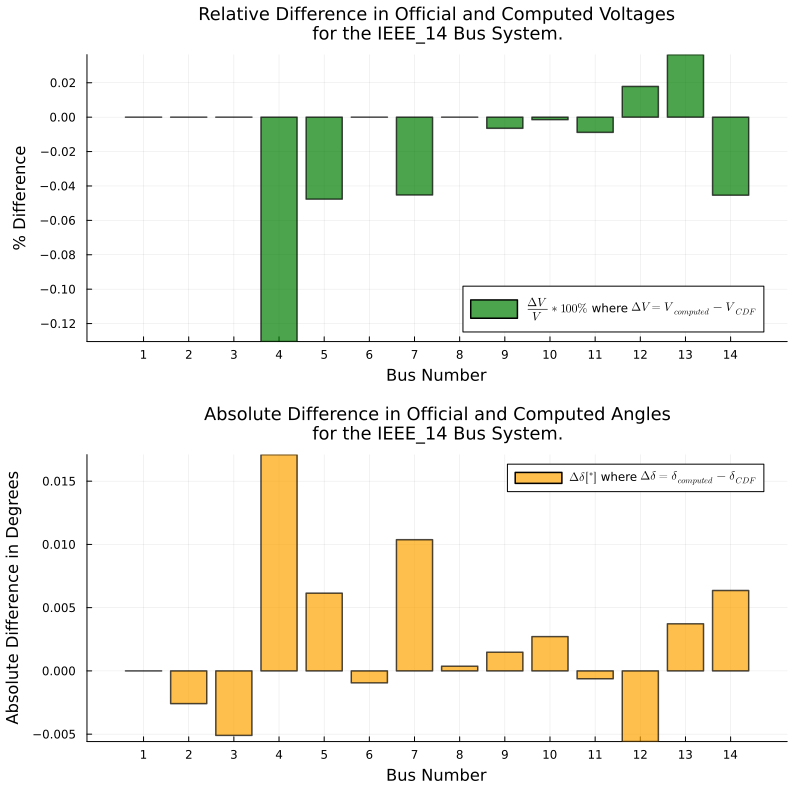
\includegraphics[width=0.3\textwidth]{\imagedir/results_IEEE_14_sparse.png}

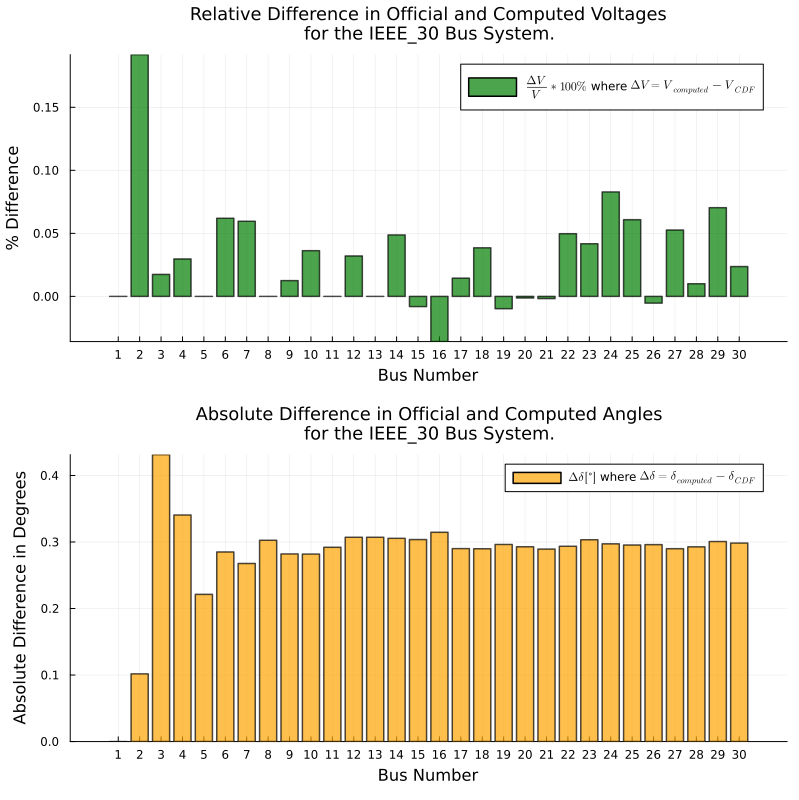
\includegraphics[width=0.3\textwidth]{\imagedir/results_IEEE_30_sparse.png}

\subsection{\cpf{}}

% \begin{figure}
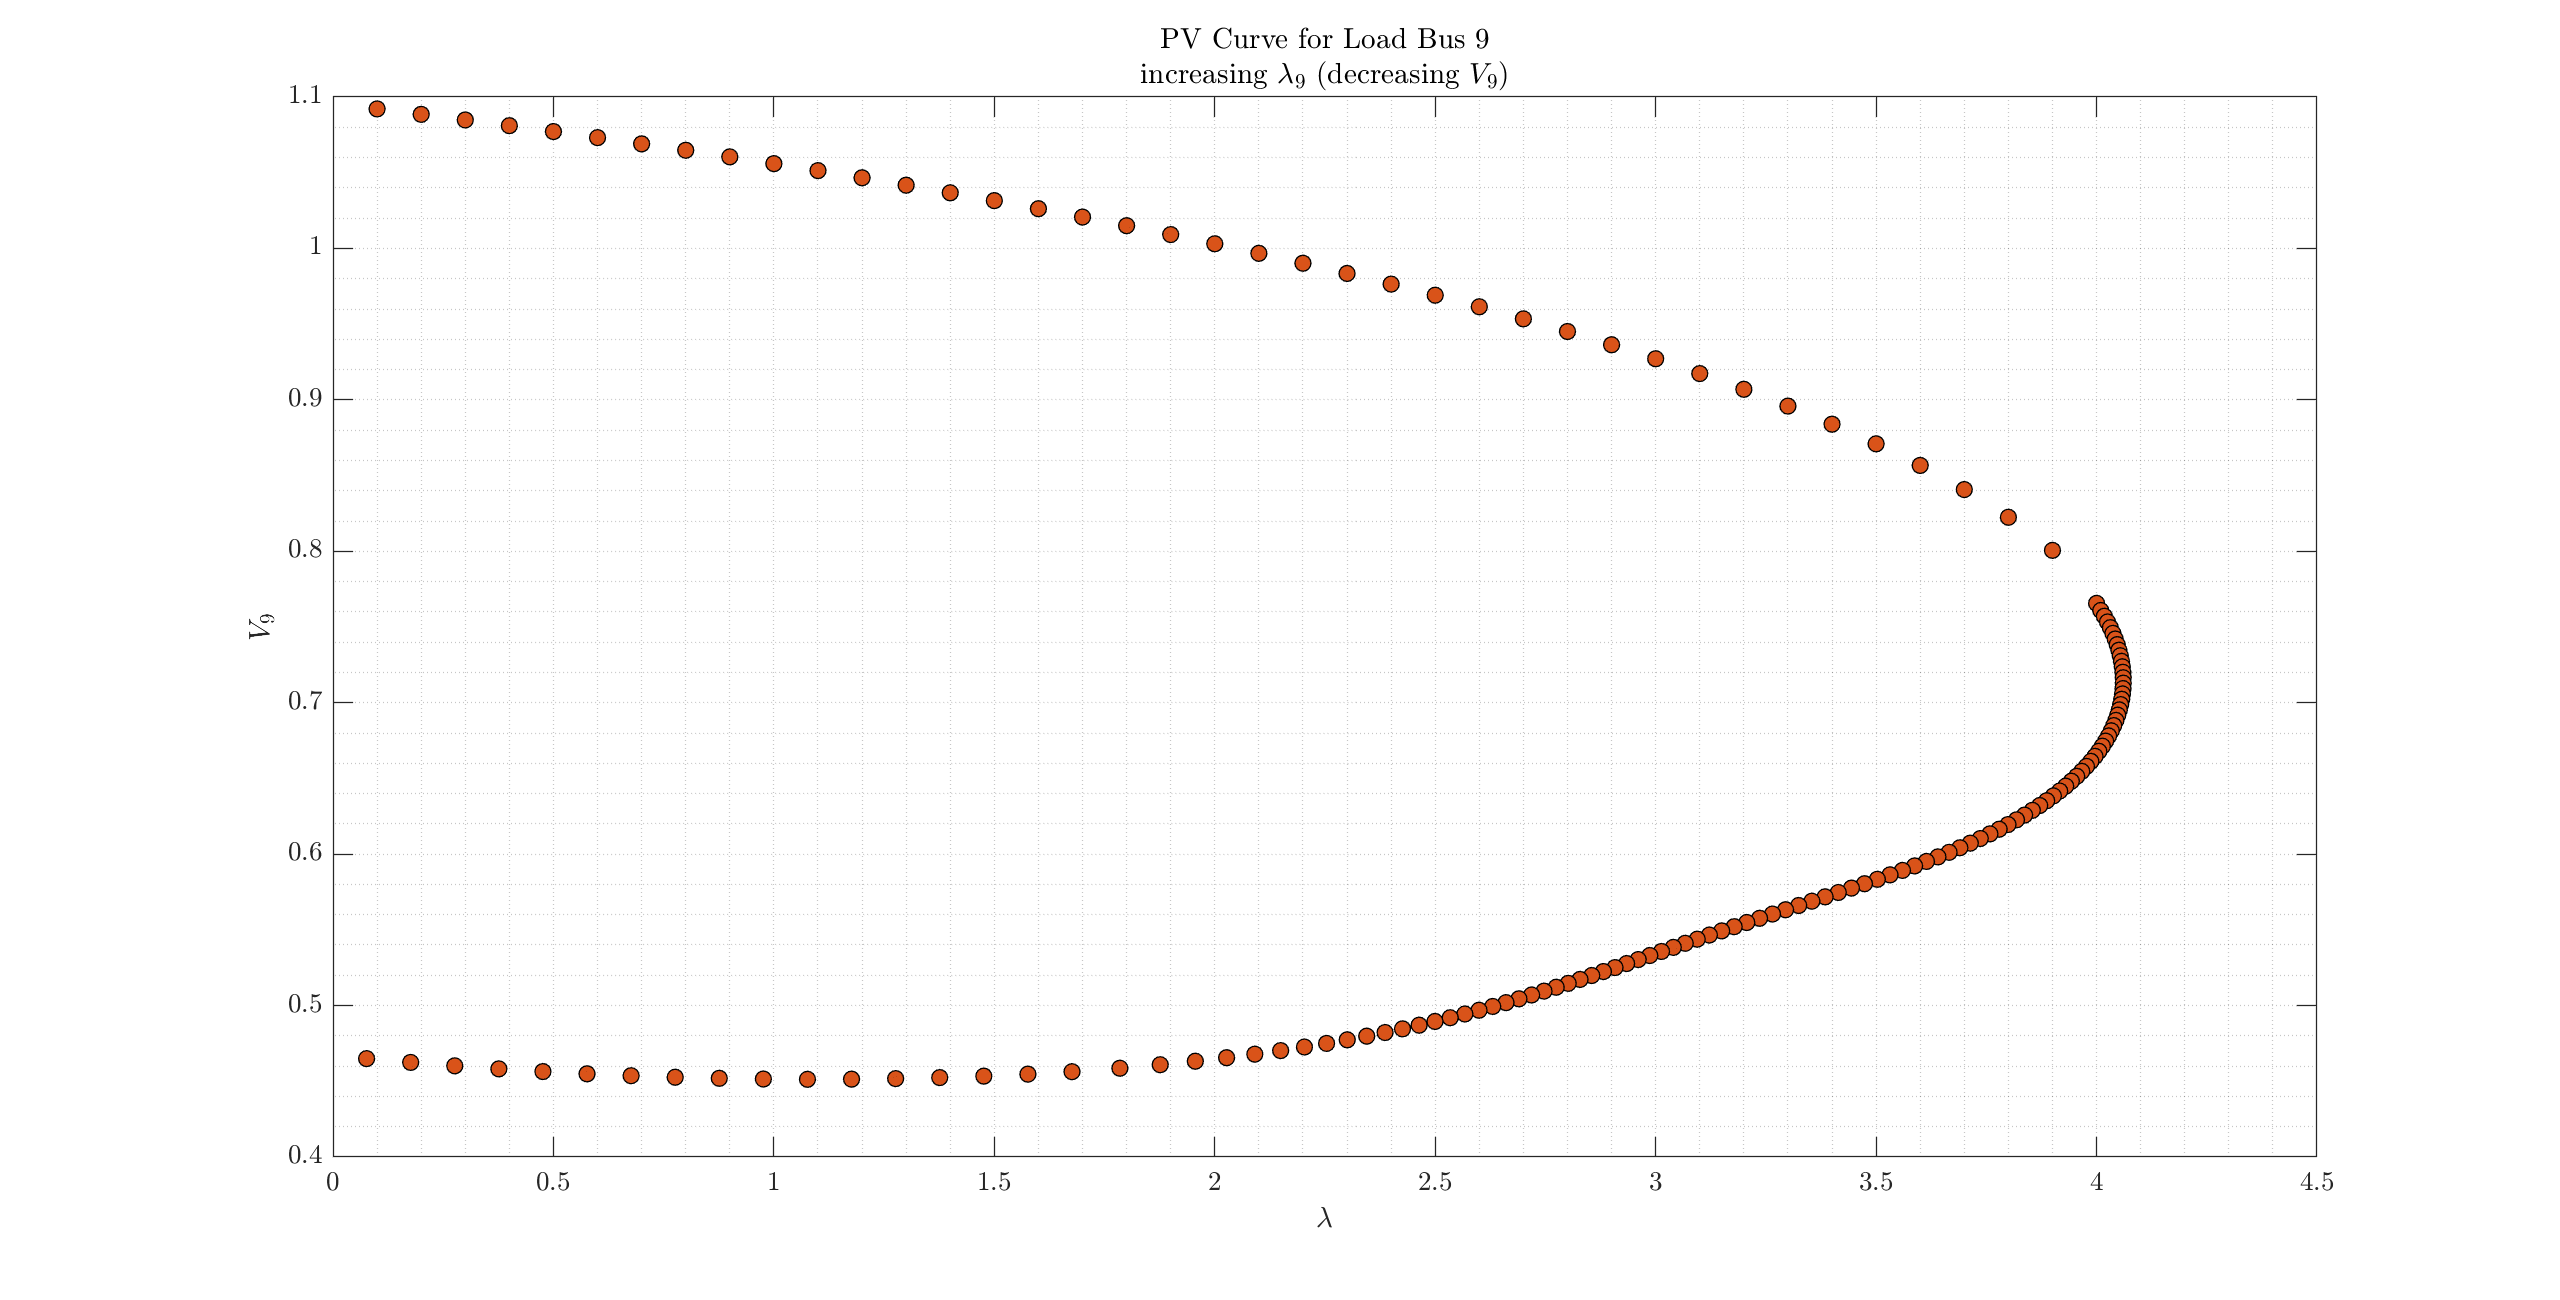
\includegraphics[width=0.5\textwidth]{\imagedir/pv09_09.png}
% \end{figure}

\subsection{\se{}}

\subsection{\opf{}}

\end{document}

\documentclass[varwidth]{standalone}

\providecommand{\packageName}[1]{PowerEdu.jl}
\providecommand{\powerflow}[1]{Power Flow}
\providecommand{\sparse}[1]{Sparse Power Flow}
\providecommand{\cpf}[1]{Continuation Power Flow}
\providecommand{\se}[1]{State Estimation}
\providecommand{\opf}[1]{Optimal Power Flow}

\usepackage{lipsum}

\begin{document}

\section{Conclusion}

\end{document}


\cite{Crow2021PowerBook,NRELSeinnaGitHub,Grainger1994PowerBook,EIAEnergyConsumptionWebpage}

% trigger a \newpage just before the given reference
% number - used to balance the columns on the last page
% adjust value as needed - may need to be readjusted if
% the document is modified later
\IEEEtriggeratref{8}
% The 'triggered' command can be changed if desired:
\IEEEtriggercmd{\enlargethispage{-5in}}

%% that's all folks
\bibliographystyle{IEEEtran}
\bibliography{BiBFile}

\end{document}


